\chapter{Mecánica cuántica para químicos: sistemas modelo}\label{ch:b3:quantum-model-systems}

Sobre una mesa de laboratorio hay tres pequeños matraces, cada uno con una disolución de un colorante
de cianina en etanol: el primero es magenta, el segundo azul, el tercero de un azul verdoso
intenso que absorbe en el rojo lejano. Las tres moléculas están construidas igual
---dos anillos nitrogenados idénticos unidos por una cadena de átomos de
carbono--- y solo difieren en la longitud de esa cadena, de dos en dos átomos de
carbono. Al alargar la cadena, el color se desplaza hacia el rojo. Un
químico de 1949 explicó la serie con uno de los problemas más sencillos de la
mecánica cuántica: un electrón libre de moverse a lo largo de una línea de longitud fija,
una ``\omterm{def:b3:quantum-model-systems:box}{partícula en una caja}''. Este capítulo monta la maquinaria que hay detrás de esa
explicación ---operadores, \omterm{def:b3:quantum-model-systems:operator}{valores propios}, la ecuación de Schrödinger--- y
resuelve los sistemas modelo que la química usa a diario: la caja, el
\omterm{def:b3:quantum-model-systems:oscillator}{oscilador armónico} de un enlace que vibra, el \omterm{def:b3:quantum-model-systems:rotor}{rotor rígido} de una molécula que
gira, el átomo de hidrógeno y la barrera que una partícula ligera puede
atravesar sin tener la energía necesaria para subirla.

\begin{recall}
El volumen del primer año mostró que la energía de un átomo está cuantizada (niveles de
energía, estados fundamental y excitados, las rayas del hidrógeno) y que un fotón
transporta $E = h\nu = hc/\lambda$. El volumen del segundo año describió un electrón mediante
una función de onda $\psi$ cuyo cuadrado es una densidad de probabilidad, separó los
orbitales del hidrógeno en partes radial y angular y contó sus nodos;
tomó como dadas las funciones de onda del hidrógeno. Aquí se deducen, en la
sección 5. De la física: la cantidad de movimiento $p = mv$ y la longitud de onda de de Broglie
$\lambda = h/p$.
\end{recall}

\begin{omfigure}
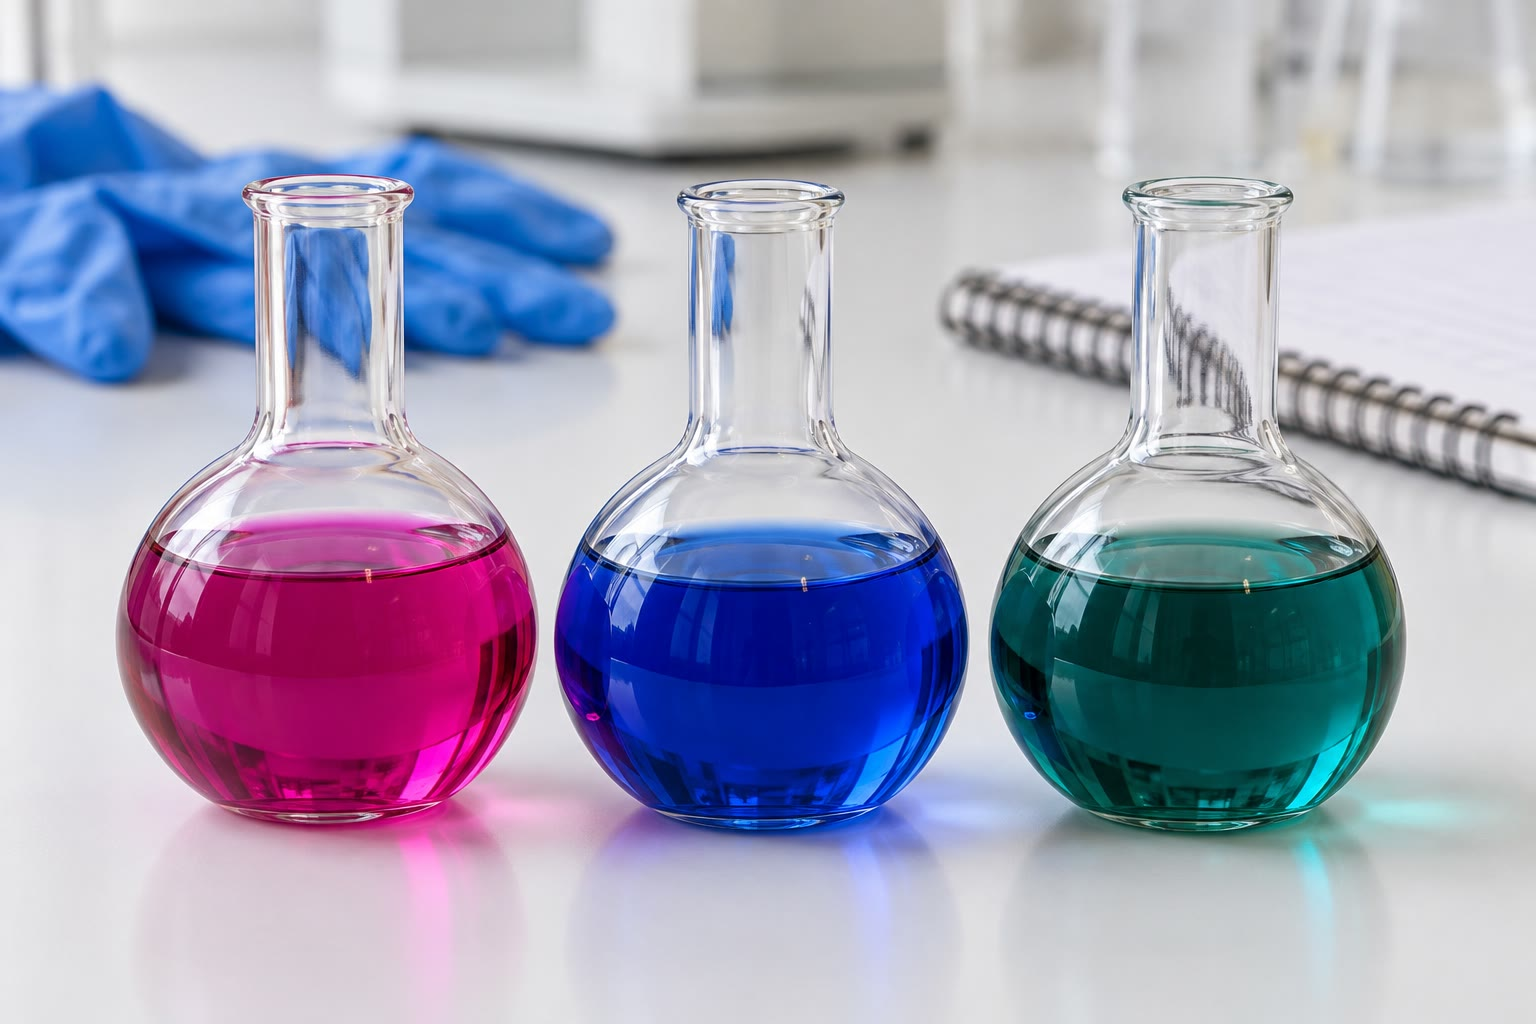
\includegraphics[width=0.62\linewidth]{images/book4/ai/b3-01-dyes.jpg}

{\small Disoluciones de tres colorantes de cianina de una misma familia. Cada par
de átomos de carbono añadido a la cadena desplaza la absorción hacia el rojo.}
\end{omfigure}

\section{Operadores, valores propios y la ecuación de Schrödinger}

La mecánica clásica asigna a una partícula una posición y una cantidad de movimiento en cada
instante. La mecánica cuántica le asigna un estado, la función de onda $\psi$, y
sustituye cada magnitud medible por una operación efectuada sobre $\psi$.

\begin{definition}[Operador, función propia, valor propio]\label{def:b3:quantum-model-systems:operator}
Un \emph{operador}\index{operador} $\hat A$ es una regla que transforma una función
en otra función: $\hat A f = g$. Es lineal si $\hat A(\lambda f +
\mu g) = \lambda\hat Af + \mu\hat Ag$. Una función no nula $f$ tal que
$\hat Af = a f$ para un número $a$ es una \emph{función propia}\index{funcion propia@función propia}
de $\hat A$, y $a$ es el \emph{valor propio}\index{valor propio} correspondiente.
\end{definition}

\begin{example}[Dos operadores: posición y cantidad de movimiento]\label{ex:b3:quantum-model-systems:xp}
En una dimensión, el \omterm{def:b3:quantum-model-systems:operator}{operador} posición multiplica por $x$, $\hat x f = xf$,
y el \omterm{def:b3:quantum-model-systems:operator}{operador} cantidad de movimiento deriva, $\hat p f = -\iu\hbar\,
\dd f/\dd x$, con $\hbar = h/2\pi$. La función $\eu^{\iu kx}$ es una
\omterm{def:b3:quantum-model-systems:operator}{función propia} de $\hat p$ con \omterm{def:b3:quantum-model-systems:operator}{valor propio} $\hbar k$: una onda de longitud de onda
$\lambda = 2\pi/k$ tiene cantidad de movimiento $h/\lambda$, la relación de de Broglie.
La función $\sin kx$ no es \omterm{def:b3:quantum-model-systems:operator}{función propia} de $\hat p$ (su derivada es
un coseno), pero sí lo es de $\hat p^2 = -\hbar^2\,\dd^2/\dd x^2$, con
\omterm{def:b3:quantum-model-systems:operator}{valor propio} $\hbar^2k^2$.
\end{example}

\begin{definition}[Operador hermítico, valor esperado]\label{def:b3:quantum-model-systems:hermitian}
Se escribe $\langle f|g\rangle = \int f^*g\,\dd\tau$ para dos funciones que se anulan
en los límites de la región. Un \omterm{def:b3:quantum-model-systems:operator}{operador} es \emph{hermítico}\index{operador hermitico@operador hermítico}
si $\langle f|\hat Ag\rangle = \langle \hat Af|g\rangle$ para todas esas
$f$ y $g$. Para un estado normalizado $\psi$ ($\langle\psi|\psi\rangle = 1$), el
\emph{valor esperado}\index{valor esperado} de $\hat A$ es
$\langle A\rangle = \langle\psi|\hat A\psi\rangle$: la media de muchas
medidas efectuadas sobre sistemas preparados de forma idéntica.
\end{definition}

Las reglas de trabajo de la química cuántica ---sus postulados--- pueden enunciarse
ahora de un tirón: toda magnitud medible está representada por un \omterm{def:b3:quantum-model-systems:hermitian}{operador
hermítico}; una medida da uno de sus \omterm{def:b3:quantum-model-systems:operator}{valores propios}; y si
$\psi$ es \omterm{def:b3:quantum-model-systems:operator}{función propia} de $\hat A$, toda medida sobre ella da el
mismo valor, su \omterm{def:b3:quantum-model-systems:operator}{valor propio}.

\begin{theorem}[Operadores hermíticos]\label{thm:b3:quantum-model-systems:hermitian-real}
Los \omterm{def:b3:quantum-model-systems:operator}{valores propios} de un \omterm{def:b3:quantum-model-systems:hermitian}{operador hermítico} son reales. Dos \omterm{def:b3:quantum-model-systems:operator}{funciones propias} con
\omterm{def:b3:quantum-model-systems:operator}{valores propios} distintos son ortogonales: $\langle f_1|f_2\rangle = 0$.
\end{theorem}

\begin{proof}
Sea $\hat Af = af$. Entonces $\langle f|\hat Af\rangle = a\langle f|f\rangle$ y
$\langle\hat Af|f\rangle = a^*\langle f|f\rangle$. El \omterm{def:b3:quantum-model-systems:operator}{operador} es \omterm{def:b3:quantum-model-systems:hermitian}{hermítico},
luego ambas cantidades son iguales, y $\langle f|f\rangle > 0$: $a = a^*$. Sean ahora $\hat Af_1
= a_1f_1$ y $\hat Af_2 = a_2f_2$ con $a_1 \ne a_2$, ambos reales. Entonces
$\langle f_1|\hat Af_2\rangle = a_2\langle f_1|f_2\rangle$ y $\langle\hat Af_1|
f_2\rangle = a_1\langle f_1|f_2\rangle$; su igualdad da $(a_2 - a_1)
\langle f_1|f_2\rangle = 0$, de donde $\langle f_1|f_2\rangle = 0$.
\end{proof}

Un valor medido es un número real, y por eso los observables deben ser
\omterm{def:b3:quantum-model-systems:hermitian}{hermíticos}; la ortogonalidad es lo que hace de los orbitales de un átomo, o de los
niveles de una caja, un conjunto limpio de estados independientes.

\begin{definition}[Conmutador]\label{def:b3:quantum-model-systems:commutator}
El \emph{conmutador}\index{conmutador} de dos \omterm{def:b3:quantum-model-systems:operator}{operadores} es $[\hat A,\hat B] =
\hat A\hat B - \hat B\hat A$. Los \omterm{def:b3:quantum-model-systems:operator}{operadores} conmutan si su conmutador es
nulo.
\end{definition}

\begin{example}[El conmutador canónico]\label{ex:b3:quantum-model-systems:canonical}
Para cualquier función $f$, $\hat x\hat pf = -\iu\hbar xf'$ y $\hat p\hat xf =
-\iu\hbar(f + xf')$. La diferencia es $[\hat x,\hat p]f = \iu\hbar f$, luego
$[\hat x,\hat p] = \iu\hbar$: la posición y la cantidad de movimiento no conmutan. Esta
única relación sustenta el principio de incertidumbre y, más abajo, todo el
espectro del \omterm{def:b3:quantum-model-systems:oscillator}{oscilador armónico}.
\end{example}

\begin{proposition}[Operadores que conmutan]\label{prop:b3:quantum-model-systems:commuting}
Si $\hat A$ y $\hat B$ conmutan y $f$ es una \omterm{def:b3:quantum-model-systems:operator}{función propia} de $\hat A$
con un \omterm{def:b3:quantum-model-systems:operator}{valor propio} no degenerado $a$, entonces $f$ es también \omterm{def:b3:quantum-model-systems:operator}{función propia} de
$\hat B$.
\end{proposition}

\begin{proof}
$\hat A(\hat Bf) = \hat B\hat Af = a(\hat Bf)$: la función $\hat Bf$ es una
\omterm{def:b3:quantum-model-systems:operator}{función propia} de $\hat A$ con el mismo \omterm{def:b3:quantum-model-systems:operator}{valor propio} $a$, o es nula. Como el
\omterm{def:b3:quantum-model-systems:operator}{valor propio} no es degenerado, $\hat Bf$ es un múltiplo de $f$, digamos $bf$.
\end{proof}

El \omterm{def:b3:quantum-model-systems:operator}{operador} de la energía es el hamiltoniano. Para una partícula de masa $m$ en un
potencial $V$, la energía clásica $p^2/2m + V$ se convierte en un \omterm{def:b3:quantum-model-systems:operator}{operador}.

\begin{definition}[Operador hamiltoniano]\label{def:b3:quantum-model-systems:schrodinger}
El \emph{operador hamiltoniano}\index{operador hamiltoniano} de una partícula de
masa $m$ que se mueve en un potencial $V(\mathbf r)$ es
\[
\hat H = -\frac{\hbar^2}{2m}\nabla^2 + V(\mathbf r), \qquad \nabla^2 =
\frac{\partial^2}{\partial x^2} + \frac{\partial^2}{\partial y^2} +
\frac{\partial^2}{\partial z^2},
\]
y, para varias partículas, la suma de sus términos cinéticos y de todas sus
energías potenciales.
\end{definition}

\begin{theorem}[La ecuación de Schrödinger]\label{thm:b3:quantum-model-systems:schrodinger}
Los estados de energía definida de un sistema ---sus estados estacionarios--- son
las \omterm{def:b3:quantum-model-systems:operator}{funciones propias} de su hamiltoniano, y sus energías permitidas son los
\omterm{def:b3:quantum-model-systems:operator}{valores propios}:
\[
\hat H\psi = E\psi,
\]
la \emph{ecuación de Schrödinger}\index{ecuacion de Schrodinger@ecuación de Schrödinger} independiente del tiempo.
Una $\psi$ aceptable es univaluada, continua y
de cuadrado integrable (puede normalizarse).
\end{theorem}
\begin{proof}[Estatus]
Es un postulado, justificado por sus consecuencias: los niveles de todos los
sistemas resueltos a continuación concuerdan con la espectroscopia. La ecuación dependiente del tiempo,
de la que esta es el caso estacionario, pertenece a la física.
\end{proof}

Son las condiciones de contorno las que cuantizan: una ecuación diferencial tiene
soluciones para cualquier $E$, pero solo un conjunto discreto de ellas se mantiene finito y
continuo. La química se reduce entonces a elegir un potencial, resolver
y leer los \omterm{def:b3:quantum-model-systems:operator}{valores propios}.

\begin{method}[Resolver un modelo unidimensional]\label{met:b3:quantum-model-systems:one-dimensional}
\begin{enumerate}
  \item Escribir el potencial $V(x)$ y el hamiltoniano; dividir el espacio en
        regiones donde $V$ sea sencillo.
  \item Resolver $-\frac{\hbar^2}{2m}\psi'' + V\psi = E\psi$ en cada región: senos
        y cosenos donde $E > V$, exponenciales reales donde $E < V$.
  \item Imponer las condiciones: $\psi = 0$ donde $V$ es infinito; $\psi$
        y $\psi'$ continuas en un escalón finito; $\psi \to 0$ en el infinito.
  \item Las condiciones solo se cumplen para ciertos valores de $E$: esos son los niveles.
  \item Normalizar cada \omterm{def:b3:quantum-model-systems:operator}{función propia}; contar sus nodos como comprobación (el
        $n$-ésimo nivel de un problema unidimensional tiene $n - 1$ nodos).
\end{enumerate}
\end{method}

\section{La partícula en una caja}

\begin{definition}[Partícula en una caja, modelo del electrón libre]\label{def:b3:quantum-model-systems:box}
Una \emph{partícula en una caja}\index{particula en una caja@partícula en una caja} se mueve libremente ($V = 0$)
entre $x = 0$ y $x = L$ y no puede salir ($V = \infty$ fuera). El
\emph{modelo del electrón libre}\index{modelo del electron libre@modelo del electrón libre} de una molécula
conjugada trata sus electrones $\pi$ como partículas independientes en una caja cuya
longitud es la de la cadena conjugada.
\end{definition}

\begin{theorem}[Niveles de la caja]\label{thm:b3:quantum-model-systems:box}
Los niveles y las \omterm{def:b3:quantum-model-systems:operator}{funciones propias} normalizadas de una partícula de masa $m$ en una caja
de longitud $L$ son
\[
E_n = \frac{n^2h^2}{8mL^2}, \qquad \psi_n(x) = \sqrt{\frac2L}\,\sin\frac{n\pi
x}{L}, \qquad n = 1, 2, 3, \dots
\]
\end{theorem}

\begin{proof}
Dentro, $\psi'' = -k^2\psi$ con $k^2 = 2mE/\hbar^2$, luego $\psi = A\sin kx +
B\cos kx$. Fuera $\psi = 0$ y la continuidad da $\psi(0) = 0$, de donde $B =
0$, y $\psi(L) = 0$, de donde $\sin kL = 0$ con $A \ne 0$: $kL = n\pi$, con $n$ un
entero positivo ($n = 0$ da $\psi = 0$; los $n$ negativos repiten las mismas
funciones). Entonces $E = \hbar^2k^2/2m = n^2\pi^2\hbar^2/2mL^2 = n^2h^2/8mL^2$.
Por último, $\int_0^L A^2\sin^2(n\pi x/L)\,\dd x = A^2L/2 = 1$ da $A =
\sqrt{2/L}$.
\end{proof}

Tres rasgos se trasladan a todo sistema ligado: la energía más baja no es
nula (la partícula nunca puede estar en reposo), los niveles se separan al crecer
$n$ y se apiñan al agrandarse la caja ($E \propto 1/L^2$): una
caja grande es casi clásica.

\begin{omfigure}
\begin{tikzpicture}
\begin{axis}[width=0.5\linewidth, height=6.4cm, xmin=-0.08, xmax=1.08,
  ymin=0, ymax=18.4, axis lines=left, xtick={0,1}, xticklabels={$0$,$L$},
  ytick={1,4,9,16}, yticklabels={$E_1$,$4E_1$,$9E_1$,$16E_1$},
  tick label style={font=\small}, xlabel={$x$}, title={\small $\psi_n$}]
\foreach \n in {1,4,9,16}{\addplot[gray!50, dashed, domain=0:1] {\n};}
\addplot[omDef, thick] table[x=x, y=p1] {figdata/out/bachelor-3-particle-in-box.dat};
\addplot[omDef, thick] table[x=x, y=p2] {figdata/out/bachelor-3-particle-in-box.dat};
\addplot[omDef, thick] table[x=x, y=p3] {figdata/out/bachelor-3-particle-in-box.dat};
\addplot[omDef, thick] table[x=x, y=p4] {figdata/out/bachelor-3-particle-in-box.dat};
\draw[very thick] (axis cs:0,0) -- (axis cs:0,18.4) (axis cs:1,0) -- (axis cs:1,18.4);
\end{axis}
\end{tikzpicture}\hspace{0.5em}%
\begin{tikzpicture}
\begin{axis}[width=0.5\linewidth, height=6.4cm, xmin=-0.08, xmax=1.08,
  ymin=0, ymax=18.4, axis lines=left, xtick={0,1}, xticklabels={$0$,$L$},
  ytick={1,4,9,16}, yticklabels={$n=1$,$n=2$,$n=3$,$n=4$},
  tick label style={font=\small}, xlabel={$x$}, title={\small $|\psi_n|^2$}]
\foreach \n in {1,4,9,16}{\addplot[gray!50, dashed, domain=0:1] {\n};}
\addplot[omThm, thick] table[x=x, y=d1] {figdata/out/bachelor-3-particle-in-box.dat};
\addplot[omThm, thick] table[x=x, y=d2] {figdata/out/bachelor-3-particle-in-box.dat};
\addplot[omThm, thick] table[x=x, y=d3] {figdata/out/bachelor-3-particle-in-box.dat};
\addplot[omThm, thick] table[x=x, y=d4] {figdata/out/bachelor-3-particle-in-box.dat};
\draw[very thick] (axis cs:0,0) -- (axis cs:0,18.4) (axis cs:1,0) -- (axis cs:1,18.4);
\end{axis}
\end{tikzpicture}

{\small Los cuatro primeros niveles de una \omterm{def:b3:quantum-model-systems:box}{partícula en una caja}, con cada función dibujada sobre
su propio nivel (en trazo discontinuo). Izquierda: $\psi_n$, con $n - 1$ nodos dentro de la caja.
Derecha: la densidad de probabilidad $|\psi_n|^2$.}
\end{omfigure}

\begin{proposition}[La caja cúbica]\label{prop:b3:quantum-model-systems:box-3d}
En una caja cúbica de arista $L$, $\psi = \psi_{n_x}(x)\psi_{n_y}(y)\psi_{n_z}(z)$ y
$E = (n_x^2 + n_y^2 + n_z^2)\,h^2/8mL^2$. Ternas distintas con la misma suma
de cuadrados dan la misma energía.
\end{proposition}

\begin{proof}
Con $V = 0$ dentro, $\hat H$ es una suma de tres \omterm{def:b3:quantum-model-systems:operator}{operadores} unidimensionales,
uno por coordenada. El producto de tres \omterm{def:b3:quantum-model-systems:operator}{funciones propias} unidimensionales es
una \omterm{def:b3:quantum-model-systems:operator}{función propia} de la suma, con la suma de los tres \omterm{def:b3:quantum-model-systems:operator}{valores propios}; se
anula en cada cara, como se exige.
\end{proof}

\begin{definition}[Niveles degenerados]\label{def:b3:quantum-model-systems:degenerate}
Las \omterm{def:b3:quantum-model-systems:operator}{funciones propias} linealmente independientes con el mismo \omterm{def:b3:quantum-model-systems:operator}{valor propio} son
\emph{niveles degenerados}\index{niveles degenerados}; su número es la
\emph{degeneración}\index{degeneracion@degeneración} $g$ de esa energía.
\end{definition}

\begin{example}[Degeneración y simetría]\label{ex:b3:quantum-model-systems:cube}
El nivel $n_x^2 + n_y^2 + n_z^2 = 6$ del cubo procede de $(2,1,1)$,
$(1,2,1)$ y $(1,1,2)$: $g = 3$. Si se estira ligeramente la caja según $z$,
la tercera función se aparta de las otras dos: la \omterm{def:b3:quantum-model-systems:degenerate}{degeneración} procedía de
la simetría del cubo. El mismo vínculo entre simetría y \omterm{def:b3:quantum-model-systems:degenerate}{degeneración}
organiza los \cref{ch:b3:point-groups,ch:b3:group-theory-applied}.
\end{example}

\subsection*{Colorantes conjugados}

En un colorante de cianina simétrico, una cadena de $j$ átomos une los dos nitrógenos
(\(j = 5\), 7, 9 para los tres colorantes de la escena inicial), y sus electrones $\pi$
están deslocalizados a lo largo de ella. Una cadena de $j$ átomos lleva $N = j + 1$ electrones
$\pi$: uno por carbono, más el par no enlazante de un nitrógeno, compartido por
todo el catión.

\begin{proposition}[Longitud de onda de absorción del electrón libre]\label{prop:b3:quantum-model-systems:free-electron}
Si $N$ electrones $\pi$ (un número par) llenan los niveles de una caja de longitud $L$,
dos por nivel, la absorción de mayor longitud de onda, del nivel lleno más alto
$n = N/2$ al siguiente, está en
\[
\lambda = \frac{8mcL^2}{h(N+1)}.
\]
\end{proposition}

\begin{proof}
$\Delta E = E_{N/2+1} - E_{N/2} = [(N/2+1)^2 - (N/2)^2]\,h^2/8mL^2 =
(N+1)\,h^2/8mL^2$, y $\lambda = hc/\Delta E$.
\end{proof}

\begin{example}[La caja desnuda falla, una caja alargada funciona]\label{ex:b3:quantum-model-systems:dyes}
% ledger: uvvis:cyanine, uvvis:carbocyanine, uvvis:dicarbocyanine, geo:C6H6.rCC
Se toma cada enlace de la cadena igual al enlace C--C del benceno,
$l = \qty{139.7}{pm}$, de modo que la cadena desnuda mide $(j - 1)l$. Para los
tres colorantes ($N = 6$, 8, 10) la fórmula da 147, 257 y 374 nm, muy
por debajo de los máximos medidos, 524, 603 y 711 nm en etanol. Los electrones
no se detienen en los nitrógenos: se extienden por los anillos. Si se alarga la
caja una longitud $\delta$ en cada extremo y se ajusta $\delta$ con el colorante central,
$\delta = \qty{222}{pm}$, alrededor de enlace y medio. El mismo $\delta$
predice entonces 474 y 732 nm para los otros dos, con un error del 10\,\% y del 3\,\%. Una sola
longitud ajustable explica una familia de colores (figura siguiente; los valores se
calculan en el script de la figura).
\end{example}

\begin{omfigure}
\begin{tikzpicture}
\begin{axis}[width=0.5\linewidth, height=5.6cm, xmin=4, xmax=10,
  ymin=0, ymax=850, xtick={5,7,9}, axis lines=left,
  xlabel={átomos $j$ de la cadena}, ylabel={$\lambda_{\max}$ / nm},
  legend cell align=left, legend style={font=\small, at={(1.03,0.5)}, anchor=west, draw=none},
  tick label style={font=\small}, label style={font=\small}]
\addplot[only marks, mark=*, omThm] table[x=j, y=measured] {figdata/out/bachelor-3-particle-in-box-dyes.dat};
\addlegendentry{medido (etanol)}
\addplot[omDef, thick, mark=square*] table[x=j, y=fitted] {figdata/out/bachelor-3-particle-in-box-dyes.dat};
\addlegendentry{caja alargada en $\delta = 222$ pm}
\addplot[gray, dashed, mark=triangle*] table[x=j, y=bare] {figdata/out/bachelor-3-particle-in-box-dyes.dat};
\addlegendentry{cadena desnuda}
\end{axis}
\end{tikzpicture}

{\small Máximos de absorción de los tres colorantes de cianina frente al
\omterm{def:b3:quantum-model-systems:box}{modelo del electrón libre}: la cadena desnuda y la caja alargada en $\delta$ en
cada extremo, con $\delta$ ajustado sobre el colorante central.}
\end{omfigure}

\begin{inthelab}[Medir una serie de colorantes]
Se pesan los tres colorantes (unos pocos miligramos), se disuelven en etanol y se
diluyen hasta que la absorbancia en el máximo quede entre 0.3 y 1. Se
registra el espectro de cada uno entre 400 y 800 nm en una cubeta de 1 cm
frente a un blanco de etanol puro, y se lee $\lambda_{\max}$ en la cima de la
banda principal. Los colorantes de cianina son sólidos que manchan e irritan: guantes, y
pesada en vitrina de gases.
\end{inthelab}

\section{El oscilador armónico}

Cerca del fondo de cualquier pozo de potencial suave, $V \approx \frac12 k(x - x_e)^2$:
las pequeñas vibraciones de un enlace, de un átomo en un cristal o de una molécula en una
jaula son todas aproximadamente armónicas.

\begin{definition}[Oscilador armónico, constante de fuerza, masa reducida, energía de punto cero]\label{def:b3:quantum-model-systems:oscillator}
Un \emph{oscilador armónico}\index{oscilador armonico@oscilador armónico} es una partícula de
masa $m$ en el potencial $V = \frac12 kx^2$; $k$ es la \emph{constante
de fuerza}\index{constante de fuerza}, y $\omega = \sqrt{k/m}$ su frecuencia
angular clásica. Una molécula diatómica de masas atómicas $m_1$, $m_2$
vibra como una sola partícula de \emph{masa reducida}\index{masa reducida}
$\mu = m_1m_2/(m_1 + m_2)$ en el potencial de su enlace. La energía del
nivel más bajo de un oscilador es su \emph{energía de punto cero}\index{energia de punto cero@energía de punto cero}.
\end{definition}

\begin{definition}[Operadores escalera]\label{def:b3:quantum-model-systems:ladder}
Con $x_0 = \sqrt{\hbar/m\omega}$, los \emph{operadores escalera}\index{operadores escalera}
son
\[
\hat a = \frac{1}{\sqrt2}\Big(\frac{\hat x}{x_0} + \frac{\iu x_0\hat p}{\hbar}\Big),
\qquad \hat a^\dagger = \frac{1}{\sqrt2}\Big(\frac{\hat x}{x_0} -
\frac{\iu x_0\hat p}{\hbar}\Big).
\]
\end{definition}

\begin{theorem}[Niveles del oscilador armónico]\label{thm:b3:quantum-model-systems:oscillator}
Los niveles de un \omterm{def:b3:quantum-model-systems:oscillator}{oscilador armónico} son
\[
E_v = \big(v + \tfrac12\big)\hbar\omega = \big(v + \tfrac12\big)h\nu, \qquad v =
0, 1, 2, \dots,
\]
equidistantes en $h\nu$, con la \omterm{def:b3:quantum-model-systems:oscillator}{energía de punto cero} $\frac12h\nu$.
\end{theorem}

\begin{proof}
A partir de $[\hat x,\hat p] = \iu\hbar$ se calcula $[\hat a,\hat a^\dagger] = 1$ y
$\hat H = \hbar\omega(\hat a^\dagger\hat a + \frac12)$. Sea $\hat N =
\hat a^\dagger\hat a$. Entonces $[\hat N,\hat a] = -\hat a$ y $[\hat N,\hat
a^\dagger] = \hat a^\dagger$: si $\hat N\psi = \nu\psi$, entonces $\hat N(\hat
a\psi) = (\nu - 1)\hat a\psi$ y $\hat N(\hat a^\dagger\psi) = (\nu + 1)\hat
a^\dagger\psi$; $\hat a$ baja el \omterm{def:b3:quantum-model-systems:operator}{valor propio} en una unidad, $\hat a^\dagger$ lo
sube. Pero $\nu = \langle\psi|\hat a^\dagger\hat a\psi\rangle/\langle\psi|\psi
\rangle = \|\hat a\psi\|^2/\|\psi\|^2 \ge 0$: el descenso debe detenerse, lo que
solo ocurre en una función con $\hat a\psi_0 = 0$, de \omterm{def:b3:quantum-model-systems:operator}{valor propio} $\nu = 0$.
Los \omterm{def:b3:quantum-model-systems:operator}{valores propios} de $\hat N$ son, por tanto, $v = 0, 1, 2, \dots$, y los de
$\hat H$ son $(v + \frac12)\hbar\omega$.
\end{proof}

\begin{proposition}[Las primeras funciones de onda]\label{prop:b3:quantum-model-systems:oscillator-functions}
En la coordenada reducida $y = x/x_0$,
\[
\psi_0 \propto \eu^{-y^2/2}, \quad \psi_1 \propto 2y\,\eu^{-y^2/2}, \quad
\psi_2 \propto (4y^2 - 2)\eu^{-y^2/2}, \quad \psi_3 \propto (8y^3 -
12y)\eu^{-y^2/2},
\]
los polinomios de Hermite multiplicados por una gaussiana. $\psi_v$ es par para $v$ par
e impar para $v$ impar.
\end{proposition}

\begin{proof}
$\hat a\psi_0 = 0$ se escribe $y\psi_0 + \dd\psi_0/\dd y = 0$, cuya solución es la
gaussiana. Cada función siguiente es $\hat a^\dagger$ aplicado a la anterior,
$\hat a^\dagger = \frac{1}{\sqrt2}(y - \dd/\dd y)$, que multiplica el
polinomio por $2y$ y le resta su derivada: $1 \to 2y \to 4y^2 - 2 \to
8y^3 - 12y$ (salvo factores). Cambiar $y$ por $-y$ cambia el signo de $y$
y de $\dd/\dd y$, de modo que $\hat a^\dagger$ invierte la paridad en cada paso.
\end{proof}

\begin{omfigure}
\begin{tikzpicture}
\begin{axis}[width=0.66\linewidth, height=6.6cm, xmin=-4, xmax=4, ymin=0,
  ymax=4.6, axis lines=left, xlabel={$y = x/x_0$},
  ylabel={energía / $\hbar\omega$}, ytick={0.5,1.5,2.5,3.5},
  tick label style={font=\small}, label style={font=\small}]
\addplot[black, thick] table[x=y, y=V] {figdata/out/bachelor-3-harmonic-oscillator.dat};
\foreach \v in {0.5,1.5,2.5,3.5}{\addplot[gray!50, dashed, domain=-4:4] {\v};}
\addplot[omDef, thick] table[x=y, y=p0] {figdata/out/bachelor-3-harmonic-oscillator.dat};
\addplot[omDef, thick] table[x=y, y=p1] {figdata/out/bachelor-3-harmonic-oscillator.dat};
\addplot[omDef, thick] table[x=y, y=p2] {figdata/out/bachelor-3-harmonic-oscillator.dat};
\addplot[omDef, thick] table[x=y, y=p3] {figdata/out/bachelor-3-harmonic-oscillator.dat};
\addplot[only marks, mark=*, mark size=1.6pt, omThm] coordinates {(-1,0.5) (1,0.5)};
\node[omThm, font=\small, anchor=west] at (axis cs:2.0,0.2) {retroceso};
\draw[omThm, ->, thin] (axis cs:2.0,0.2) -- (axis cs:1.08,0.47);
\end{axis}
\end{tikzpicture}

{\small El potencial armónico, sus cuatro primeros niveles y sus funciones de onda,
cada una dibujada sobre su nivel. Las funciones de onda llegan más allá de los
puntos de retroceso clásicos ($y = \pm1$ para $v = 0$, puntos rojos), donde una partícula
clásica se detendría.}
\end{omfigure}

\begin{example}[Energías de punto cero de \ce{H2} y \ce{D2}]\label{ex:b3:quantum-model-systems:zpe}
% ledger: diat:H2.we, diat:D2.we
Los números de onda armónicos son $\tilde\omega_e = \qty{4401.2}{cm^{-1}}$ para
\ce{H2} y \qty{3115.5}{cm^{-1}} para \ce{D2}, en la razón $1.413$, próxima a
$\sqrt2$: mismo enlace y misma \omterm{def:b3:quantum-model-systems:oscillator}{constante de fuerza}, \omterm{def:b3:quantum-model-systems:oscillator}{masa reducida} doble. Las
\omterm{def:b3:quantum-model-systems:oscillator}{energías de punto cero} armónicas son la mitad, 2200.6 y \qty{1557.8}{cm^{-1}},
\qty{26.3}{kJ/mol} y \qty{18.6}{kJ/mol}. Una molécula nunca puede perder esta
energía; la diferencia entre isótopos es el origen de los efectos isotópicos
de los \cref{ch:b3:statistical-thermo-applied,ch:b3:rate-theories}.
\end{example}

\section{El rotor rígido}

Una molécula diatómica también gira en torno a su centro de masas. Tratada como dos
masas a una distancia fija $r$, es un \omterm{def:b3:quantum-model-systems:rotor}{rotor rígido} de momento de inercia
$I = \mu r^2$, la \omterm{def:b3:quantum-model-systems:oscillator}{masa reducida} a la distancia $r$ del eje.

\begin{definition}[Rotor rígido, armónicos esféricos]\label{def:b3:quantum-model-systems:rotor}
Un \emph{rotor rígido}\index{rotor rigido@rotor rígido} es un cuerpo de forma fija que gira
libremente; para una molécula lineal, $\hat H = \hat L^2/2I$, donde $\hat L^2$ es el
\omterm{def:b3:quantum-model-systems:operator}{operador} del cuadrado del momento angular. Sus \omterm{def:b3:quantum-model-systems:operator}{funciones propias}, que
solo dependen de los ángulos $\theta$ y $\phi$, son los \emph{armónicos
esféricos}\index{armonicos esfericos@armónicos esféricos} $Y_{l,m}(\theta,\phi)$, indexados por $l =
0, 1, 2, \dots$ y $m = -l, \dots, l$; para una molécula, $l$ se escribe $J$.
\end{definition}

El rotor en un anillo (rotación en un plano, en torno a un eje fijo) se resuelve
primero; contiene lo esencial.

\begin{theorem}[El anillo]\label{thm:b3:quantum-model-systems:ring}
Una partícula de momento de inercia $I$ que gira en un plano tiene los niveles
$E_m = m^2\hbar^2/2I$ con $m = 0, \pm1, \pm2, \dots$; todos los niveles salvo $m = 0$
son doblemente degenerados.
\end{theorem}

\begin{proof}
La única coordenada es el ángulo $\phi$, y $\hat H = -(\hbar^2/2I)\,
\dd^2/\dd\phi^2$. Las soluciones de $\psi'' = -(2IE/\hbar^2)\psi$ son $\eu^{\iu
m\phi}$ con $m^2 = 2IE/\hbar^2$. Una función univaluada debe tomar el mismo
valor en $\phi$ y en $\phi + 2\pi$: $\eu^{2\pi\iu m} = 1$, luego $m$ es entero.
Las funciones con $m$ y $-m$ tienen la misma energía y son independientes.
\end{proof}

\begin{theorem}[Niveles del rotor rígido]\label{thm:b3:quantum-model-systems:rotor}
$\hat L^2Y_{J,m} = J(J+1)\hbar^2\,Y_{J,m}$ y $\hat L_zY_{J,m} = m\hbar\,
Y_{J,m}$, de modo que los niveles de un \omterm{def:b3:quantum-model-systems:rotor}{rotor rígido} lineal son
\[
E_J = \frac{\hbar^2}{2I}\,J(J+1), \qquad J = 0, 1, 2, \dots,
\]
cada uno con \omterm{def:b3:quantum-model-systems:degenerate}{degeneración} $g_J = 2J + 1$.
\end{theorem}
\admitted

La demostración general, mediante \omterm{def:b3:quantum-model-systems:ladder}{operadores escalera} del momento angular, corresponde a
cursos más avanzados; he aquí una comprobación. En coordenadas esféricas,
\[
\hat L^2 = -\hbar^2\Big[\frac{1}{\sin\theta}\frac{\partial}{\partial\theta}
\Big(\sin\theta\frac{\partial}{\partial\theta}\Big) +
\frac{1}{\sin^2\theta}\frac{\partial^2}{\partial\phi^2}\Big].
\]
Para $Y_{1,0} \propto \cos\theta$, el corchete vale $\frac{1}{\sin\theta}(-2\sin\theta
\cos\theta) = -2\cos\theta$, luego $\hat L^2Y_{1,0} = 2\hbar^2Y_{1,0} = 1(1+1)\hbar^2
Y_{1,0}$. Para $Y_{1,\pm1} \propto \sin\theta\,\eu^{\pm\iu\phi}$ el mismo
cálculo vuelve a dar $2\hbar^2$, y $\hat L_z = -\iu\hbar\,\partial/\partial
\phi$ da $\pm\hbar$.

\begin{proposition}[Armónicos esféricos reales]\label{prop:b3:quantum-model-systems:real-harmonics}
Para $l = 1$, las combinaciones $Y_{1,0}$, $(Y_{1,-1} - Y_{1,1})/\sqrt2$ e
$\iu(Y_{1,-1} + Y_{1,1})/\sqrt2$ son reales y proporcionales a $z/r$, $x/r$ e
$y/r$; para $l = 2$ la misma construcción da funciones proporcionales a
$(3z^2 - r^2)$, $xz$, $yz$, $xy$ y $x^2 - y^2$, divididas por $r^2$.
\end{proposition}

\begin{proof}
$Y_{1,\pm1} \propto \mp\sin\theta\,\eu^{\pm\iu\phi}$ con el convenio de signos
habitual, de modo que su diferencia dividida por $\sqrt2$ es $\propto\sin\theta\cos\phi =
x/r$ y la suma ponderada con $\iu$ es $\propto\sin\theta\sin\phi = y/r$;
$\cos\theta = z/r$. Toda combinación de \omterm{def:b3:quantum-model-systems:operator}{funciones propias} degeneradas sigue siendo
\omterm{def:b3:quantum-model-systems:operator}{función propia} de $\hat L^2$ (con el mismo $l$), aunque ya no de $\hat
L_z$. El caso $l = 2$ es el mismo álgebra con $\sin^2\theta\,\eu^{\pm2\iu\phi}$
y $\sin\theta\cos\theta\,\eu^{\pm\iu\phi}$.
\end{proof}

Son las partes angulares de los orbitales $p$ y $d$ dibujados en el volumen del segundo
año: sus nombres $p_x$, $d_{xy}$, $d_{z^2}$ son las formas cartesianas que acaban de
encontrarse.

\begin{omfigure}
\begin{tikzpicture}[font=\small]
  \draw[->] (0,-0.2) -- (0,5.4) node[above] {$E/(\hbar^2/2I)$};
  \foreach \J/\E/\g in {0/0/1,1/2/3,2/6/5,3/12/7}{
    \pgfmathsetmacro{\y}{0.4*\E+0.1}
    \draw[omstate] (0.6,\y) -- (3.0,\y);
    \node[anchor=east] at (0.55,\y) {$\E$};
    \node[anchor=west] at (3.1,\y) {$J = \J$, \ $g = \g$};
  }
  \draw[<->, omThm] (2.4,0.9) -- (2.4,2.5) node[midway, left] {$4$};
  \draw[<->, omThm] (1.4,0.1) -- (1.4,0.9) node[midway, left] {$2$};
\end{tikzpicture}

{\small Los primeros niveles de un \omterm{def:b3:quantum-model-systems:rotor}{rotor rígido} lineal, $E_J = J(J+1)\,\hbar^2/2I$,
con sus \omterm{def:b3:quantum-model-systems:degenerate}{degeneraciones} $2J + 1$. Las separaciones crecen como $2(J+1)$: es la razón
de las rayas equidistantes del \cref{ch:b3:rovibrational-spectroscopy}.}
\end{omfigure}

\begin{example}[Niveles de rotación de \ce{HCl}]\label{ex:b3:quantum-model-systems:hcl}
% ledger: diat:HCl.Be
Los espectroscopistas escriben $E_J = hcB\,J(J+1)$ con la constante de rotación $B =
\hbar/(4\pi cI)$ en números de onda. Para \ce{H^{35}Cl}, $B = \qty{10.593}{cm^{-1}}$:
los primeros niveles están en 0, 21.19, 63.56 y \qty{127.12}{cm^{-1}}, todos muy
por debajo de la energía térmica a temperatura ambiente, $kT/hc = \qty{207}{cm^{-1}}$.
Hay muchos niveles de rotación poblados; de vibración, solo uno
($\tilde\omega_e = \qty{2991}{cm^{-1}}$).
\end{example}

\section{El átomo de hidrógeno y el efecto túnel}

\subsection*{El átomo de hidrógeno, resuelto}

Un electrón de carga $-e$ en torno a un núcleo de carga $+e$ tiene $V = -e^2/
4\pi\varepsilon_0r$. Con la \omterm{def:b3:quantum-model-systems:oscillator}{masa reducida} $\mu$ del electrón y el protón,
\[
\hat H = -\frac{\hbar^2}{2\mu}\nabla^2 - \frac{e^2}{4\pi\varepsilon_0r},\qquad
\nabla^2 = \frac{1}{r^2}\frac{\partial}{\partial r}\Big(r^2\frac{\partial}{
\partial r}\Big) - \frac{\hat L^2}{\hbar^2r^2}.
\]
La parte angular de $\nabla^2$ es el \omterm{def:b3:quantum-model-systems:operator}{operador} del rotor: las soluciones se
separan en la forma $\psi = R(r)\,Y_{l,m}(\theta,\phi)$, y $R$ obedece a la ecuación
radial
\[
-\frac{\hbar^2}{2\mu}\frac{1}{r^2}\frac{\dd}{\dd r}\Big(r^2\frac{\dd R}{\dd r}
\Big) + \Big[\frac{l(l+1)\hbar^2}{2\mu r^2} - \frac{e^2}{4\pi\varepsilon_0r}
\Big]R = ER.
\]
La rotación añade un término centrífugo $l(l+1)\hbar^2/2\mu r^2$ que mantiene
a los electrones con $l > 0$ alejados del núcleo.

\begin{theorem}[Niveles del átomo de hidrógeno]\label{thm:b3:quantum-model-systems:hydrogen}
Los niveles ligados de un átomo hidrogenoide de carga nuclear $Ze$ son
\[
E_n = -\frac{\mu}{m_e}\,\frac{Z^2hcR_\infty}{n^2}, \qquad n = 1, 2, \dots,
\quad hcR_\infty = \frac{m_ee^4}{8\varepsilon_0^2h^2},
\]
con $l = 0, \dots, n - 1$; las funciones radiales $1s$ y $2p$ son $R_{10}
\propto \eu^{-Zr/a}$ y $R_{21} \propto r\,\eu^{-Zr/2a}$, con $a =
(m_e/\mu)a_0$.
\end{theorem}

\begin{proof}[Demostración parcial]
Se toma $Z = 1$ y se ensaya $R = \eu^{-r/a}$ con $l = 0$. Entonces $R' = -R/a$ y
$\frac{1}{r^2}(r^2R')' = R/a^2 - 2R/(ar)$. La ecuación radial se convierte en
$-\frac{\hbar^2}{2\mu}\big(\frac{1}{a^2} - \frac{2}{ar}\big) - \frac{e^2}{4\pi
\varepsilon_0r} = E$ para todo $r$: los términos en $1/r$ se cancelan si $a =
4\pi\varepsilon_0\hbar^2/\mu e^2$, y entonces $E = -\hbar^2/2\mu a^2 = -\mu
e^4/8\varepsilon_0^2h^2$, el nivel $n = 1$. Con $R = r\eu^{-r/b}$ y $l = 1$,
la misma sustitución deja términos en $1/r^2$ (que se cancelan con el
término centrífugo), en $1/r$ (que se cancelan si $b = 2a$) y una constante, $E =
-\hbar^2/2\mu b^2$, la cuarta parte de la anterior: el nivel $n = 2$. El caso
general, un polinomio multiplicado por $\eu^{-r/na}$ cuya serie debe terminar para seguir siendo
normalizable, corresponde a cursos más avanzados.
\end{proof}

\begin{omfigure}
\begin{tikzpicture}
\begin{axis}[width=0.66\linewidth, height=5.4cm, xmin=0, xmax=12,
  ymin=-0.15, ymax=1.05, axis lines=left, samples=160, domain=0:12,
  xlabel={$r/a$}, ylabel={$R(r)$, a escala},
  legend cell align=left, legend style={font=\small, draw=none}, tick label style={font=\small},
  label style={font=\small}]
\addplot[omDef, thick] {exp(-x)}; \addlegendentry{$R_{10} \propto \eu^{-r/a}$}
\addplot[omThm, thick] {(1-x/2)*exp(-x/2)}; \addlegendentry{$R_{20} \propto (1 - r/2a)\eu^{-r/2a}$}
\addplot[omProp, thick] {0.5*x*exp(-x/2)/exp(-1)}; \addlegendentry{$R_{21} \propto r\,\eu^{-r/2a}$}
\addplot[gray, dashed] {0};
\end{axis}
\end{tikzpicture}

{\small Funciones radiales del átomo de hidrógeno, obtenidas de las soluciones anteriores
(cada una escalada a un máximo próximo a 1). $R_{20}$ tiene un nodo radial en $r = 2a$;
$R_{21}$ se anula en el núcleo, expulsada por el término centrífugo.}
\end{omfigure}

\begin{example}[La energía de ionización del hidrógeno]\label{ex:b3:quantum-model-systems:ie}
% ledger: const:RyhcEV, const:me, const:mp
$hcR_\infty = \qty{13.6057}{eV}$ y $\mu/m_e = 1/(1 + m_e/m_p) = 0.999456$, luego
$-E_1 = \qty{13.598}{eV}$: la energía de ionización medida del hidrógeno, hasta la
última cifra dada en el volumen del primer año. La \omterm{def:b3:quantum-model-systems:oscillator}{masa reducida} cambia la cuarta
cifra significativa.
\end{example}

\subsection*{Efecto túnel}

\begin{definition}[Efecto túnel, probabilidad de transmisión]\label{def:b3:quantum-model-systems:tunnelling}
Se llama \emph{efecto túnel}\index{efecto tunel@efecto túnel} al paso de una partícula a través de una
región en la que su energía es inferior a la energía potencial, prohibido en
mecánica clásica. La \emph{probabilidad de transmisión}\index{probabilidad de transmision@probabilidad de transmisión}
$T$ de una barrera es la fracción de partículas incidentes que se encuentran
más allá de ella.
\end{definition}

\begin{proposition}[Barreras delgadas y gruesas]\label{prop:b3:quantum-model-systems:barrier}
Dentro de una barrera de altura $V_0 > E$, $\psi$ es una combinación de
$\eu^{\pm\kappa x}$ con $\kappa = \sqrt{2m(V_0 - E)}/\hbar$. Para una barrera
rectangular de anchura $a$,
\[
T = \Big[1 + \frac{\sinh^2(\kappa a)}{4\varepsilon(1-\varepsilon)}\Big]^{-1},
\qquad \varepsilon = \frac{E}{V_0},
\]
y para una barrera gruesa ($\kappa a \gg 1$), $T \approx 16\varepsilon(1-\varepsilon)
\,\eu^{-2\kappa a}$.
\end{proposition}

\begin{proof}[Demostración parcial]
En la barrera, la \omterm{thm:b3:quantum-model-systems:schrodinger}{ecuación de Schrödinger} se escribe $\psi'' = \kappa^2\psi$, cuyas
soluciones son las dos exponenciales. Empalmar $\psi$ y $\psi'$ en las dos
paredes con las ondas $\eu^{\pm\iu kx}$ del exterior da cuatro ecuaciones lineales; su
solución, una página de álgebra, es la fórmula de $T$, que se admite. Para
$\kappa a$ grande, $\sinh\kappa a \approx \frac12\eu^{\kappa a}$ domina y
da la forma de barrera gruesa.
\end{proof}

El factor decisivo es $\eu^{-2\kappa a}$, y $\kappa \propto \sqrt m$:
el \omterm{def:b3:quantum-model-systems:tunnelling}{efecto túnel} es cosa de las partículas más ligeras, los electrones primero, luego
los protones, y mucho menos los deuterones.

\begin{omfigure}
\begin{tikzpicture}
\begin{axis}[width=0.66\linewidth, height=5.6cm, xmin=0, xmax=1, ymode=log,
  ymin=1e-10, ymax=1e-1, axis lines=left, xlabel={$E/V_0$},
  ylabel={probabilidad de transmisión $T$},
  legend cell align=left, legend style={font=\small, at={(0.03,0.97)}, anchor=north west, draw=none},
  tick label style={font=\small}, label style={font=\small}]
\addplot[omDef, thick] table[x=eps, y=TH] {figdata/out/bachelor-3-tunnelling.dat};
\addlegendentry{protón}
\addplot[omThm, thick, dashed] table[x=eps, y=TD] {figdata/out/bachelor-3-tunnelling.dat};
\addlegendentry{deuterón}
\end{axis}
\end{tikzpicture}

{\small \omterm{def:b3:quantum-model-systems:tunnelling}{Probabilidad de transmisión} a través de una barrera modelo de 0.40 eV de altura y
50 pm de anchura. A la mitad de la altura de la barrera, el protón pasa unas 58 veces
más a menudo que el deuterón (escala logarítmica).}
\end{omfigure}

\begin{remark}[Dónde se manifiesta el efecto túnel]\label{rem:b3:quantum-model-systems:where}
La molécula de amoniaco se invierte como un paraguas, con su nitrógeno atravesando el
plano de los tres hidrógenos, por \omterm{def:b3:quantum-model-systems:tunnelling}{efecto túnel} a través de una barrera baja; las transferencias
de protón y de átomo de hidrógeno en las enzimas muestran efectos isotópicos cinéticos mucho
mayores de lo que predice el \cref{ch:b3:rate-theories} sin \omterm{def:b3:quantum-model-systems:tunnelling}{efecto túnel}; y el
microscopio de \omterm{def:b3:quantum-model-systems:tunnelling}{efecto túnel} obtiene imágenes de átomos individuales sobre una superficie gracias a la
corriente de electrones que atraviesan por \omterm{def:b3:quantum-model-systems:tunnelling}{efecto túnel} un hueco de vacío de unas décimas de
nanómetro, una corriente que se divide por diez por cada 0.1 nm adicional.
\end{remark}

\begin{history}[Schrödinger, 1926]
\begin{minipage}[t]{0.72\linewidth}
En cuatro artículos escritos en la primera mitad de 1926, Erwin Schrödinger
sustituyó las reglas cuánticas del átomo de Bohr por una ecuación de ondas, la resolvió para
el átomo de hidrógeno, el oscilador y el rotor, y recuperó los niveles
que la espectroscopia había medido. Los enteros que Bohr había impuesto a mano
aparecían ahora por sí solos, con la misma naturalidad que el número de nodos de una
cuerda que vibra.
Compartió el premio Nobel de Física de 1933 con Paul Dirac.
\end{minipage}\hfill
\begin{minipage}[t]{0.22\linewidth}\vspace{0pt}
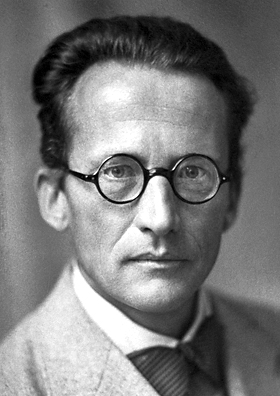
\includegraphics[width=\linewidth]{images/book4/schrodinger-1933.jpg}\par
{\footnotesize Schrödinger en 1933.}
\end{minipage}
\end{history}

\section{Ejercicios}

\begin{exercise}[$\star$]\label{exo:b3:quantum-model-systems:1}
Un electrón está confinado en una caja de longitud (a) \qty{1.00}{nm}, (b)
\qty{0.50}{nm}. Calcúlese $E_1$ en julios y en electronvoltios, y la longitud de onda
de la transición $n = 1 \to 2$.
\end{exercise}

\begin{exercise}[$\star$]\label{exo:b3:quantum-model-systems:2}
Enumérense los cinco niveles más bajos de una \omterm{def:b3:quantum-model-systems:box}{partícula en una caja} cúbica, en unidades de
$h^2/8mL^2$, con sus \omterm{def:b3:quantum-model-systems:degenerate}{degeneraciones}.
\end{exercise}

\begin{exercise}[$\star$]\label{exo:b3:quantum-model-systems:3}
Calcúlense los \omterm{def:b3:quantum-model-systems:commutator}{conmutadores} $[\hat x^2,\hat p]$ y $[\hat p^2,\hat x]$ haciéndolos actuar
sobre una función $f(x)$.
\end{exercise}

\begin{exercise}[$\star$]\label{exo:b3:quantum-model-systems:4}
% ledger: diat:HCl.Be
Con $B = \qty{10.593}{cm^{-1}}$ para \ce{H^{35}Cl}, dense las energías (en
\unit{cm^{-1}}) y las \omterm{def:b3:quantum-model-systems:degenerate}{degeneraciones} de los niveles $J = 0$ a 3, y el momento de
inercia de la molécula.
\end{exercise}

\begin{exercise}[$\star\star$]\label{exo:b3:quantum-model-systems:5}
Para el estado $\psi_n$ de una \omterm{def:b3:quantum-model-systems:box}{partícula en una caja}, calcúlense $\langle x\rangle$ y
$\langle x^2\rangle$. Evalúese $\langle x^2\rangle$ para $n = 1$ y compárese con
el valor clásico $L^2/3$ de una partícula con igual probabilidad de estar en cualquier punto.
\end{exercise}

\begin{exercise}[$\star\star$]\label{exo:b3:quantum-model-systems:6}
% ledger: diat:H2.we, diat:D2.we
Calcúlense las \omterm{def:b3:quantum-model-systems:oscillator}{energías de punto cero} armónicas de \ce{H2} y \ce{D2} en
\unit{kJ/mol} a partir de $\tilde\omega_e = \qty{4401.2}{cm^{-1}}$ y
\qty{3115.5}{cm^{-1}}, y su diferencia. ¿Qué razón de números de onda cabe
esperar de las \omterm{def:b3:quantum-model-systems:oscillator}{masas reducidas}, y cuánto se acerca a ella la medida?
\end{exercise}

\begin{exercise}[$\star\star$]\label{exo:b3:quantum-model-systems:7}
La función $\phi = Nx(L - x)$ es una aproximación burda del estado fundamental de la
caja. Normalícese y calcúlese después su solapamiento $\langle\psi_1|\phi\rangle$ con
el verdadero estado fundamental.
\end{exercise}

\begin{exercise}[$\star\star$]\label{exo:b3:quantum-model-systems:8}
Demuéstrese que $\hat p = -\iu\hbar\,\dd/\dd x$ es \omterm{def:b3:quantum-model-systems:hermitian}{hermítico} para funciones que
se anulan en los extremos de un intervalo, y que $\hat x\hat p$ no lo es.
\end{exercise}

\begin{exercise}[$\star\star$]\label{exo:b3:quantum-model-systems:9}
Modélese el hexa-1,3,5-trieno como seis electrones $\pi$ en una caja de longitud $6l$, $l =
\qty{139.7}{pm}$ (cinco enlaces y medio enlace en cada extremo). Predígase la
longitud de onda de su primera absorción. ¿Es coloreada la molécula?
\end{exercise}

\begin{exercise}[$\star\star\star$]\label{exo:b3:quantum-model-systems:10}
Para la barrera modelo de la figura ($V_0 = \qty{0.40}{eV}$, $a = \qty{50}{pm}$)
en $E = V_0/2$, calcúlese $\kappa$ para un protón y para un deuterón y, con la
fórmula de barrera gruesa, la razón $T_H/T_D$. Compárese con la razón exacta, 58.
\end{exercise}

\begin{exercise}[$\star\star\star$]\label{exo:b3:quantum-model-systems:11}
Trátense los seis electrones $\pi$ del benceno como partículas en un anillo de radio
\qty{139.7}{pm} (la distancia C--C es igual al radio de un hexágono regular).
Llénense los niveles y calcúlese después la longitud de onda de la transición del
nivel lleno más alto al nivel vacío más bajo.
\end{exercise}

\begin{exercise}[$\star\star\star$]\label{exo:b3:quantum-model-systems:12}
Para el estado $1s$ del hidrógeno, $\psi = (\pi a^3)^{-1/2}\eu^{-r/a}$. Calcúlense los
\omterm{def:b3:quantum-model-systems:hermitian}{valores esperados} $\langle r\rangle$ y $\langle V\rangle$, y compruébese que
$\langle V\rangle = 2E_1$. (Úsese $\int_0^\infty r^n\eu^{-\beta r}\dd r =
n!/\beta^{n+1}$.)
\end{exercise}

\section{Problema: ¿cuánto mide un colorante?}

\begin{problem}[{Problema de fin de semana --- el modelo del electrón libre de tres
colorantes de cianina: por qué falla una cadena desnuda, qué transiciones están permitidas, las
escalas de energía de una molécula y la longitud de caja que se ajusta}]
\label{pb:b3:quantum-model-systems:1}
% ledger: uvvis:cyanine, uvvis:carbocyanine, uvvis:dicarbocyanine, geo:C6H6.rCC, diat:HCl.we, diat:HCl.Be
Tres colorantes de cianina simétricos absorben a 524, 603 y 711 nm en etanol; sus
cadenas conjugadas, entre los dos nitrógenos y contándolos, tienen $j = 5$, 7
y 9 átomos. Se toma cada enlace igual a $l = \qty{139.7}{pm}$, $m_e =
\qty{9.109e-31}{kg}$, $h = \qty{6.626e-34}{J.s}$, $c = \qty{2.998e8}{m/s}$,
$k = \qty{1.381e-23}{J/K}$, $\qty{1}{eV} = \qty{1.602e-19}{J}$.

\medskip\noindent\textbf{Parte I --- Una cadena desnuda.}
\begin{enumerate}
  \item Explíquese por qué una cadena de $j$ átomos lleva $N = j + 1$ electrones $\pi$, y
        dese $N$ para cada colorante.
  \item ¿Qué niveles de la caja son el lleno más alto y el vacío más bajo
        para el primer colorante?
  \item Demuéstrese que la primera absorción está en $\lambda = 8mcL^2/h(N+1)$.
  \item Dese la longitud desnuda $L_0 = (j - 1)l$ de cada cadena.
  \item Calcúlese $\lambda$ para cada colorante con $L = L_0$.
  \item Compárese con los valores medidos. ¿En qué sentido se equivoca el modelo
        y qué indica eso sobre $L$?
\end{enumerate}

\medskip\noindent\textbf{Parte II --- Qué transiciones están permitidas.}
La intensidad de una transición $n \to n'$ es proporcional a $|\langle
\psi_n|x - L/2|\psi_{n'}\rangle|^2$.
\begin{enumerate}[resume]
  \item Demuéstrese que $\psi_n$ es simétrica respecto del centro de la caja para $n$
        impar y antisimétrica para $n$ par.
  \item Dedúzcase que la integral se anula cuando $n + n'$ es par.
  \item ¿Está permitida la transición HOMO $\to$ LUMO de cada colorante?
  \item Para el segundo colorante, ¿está permitida la transición del HOMO al nivel
        situado encima del LUMO? ¿Y la del nivel situado debajo del HOMO al LUMO?
  \item En el modelo, ¿a qué longitud de onda (como fracción de la primera)
        estaría la siguiente transición permitida desde el HOMO?
  \item ¿Por qué una regla así, deducida solo de la simetría, sobrevive a lo
        burdo del modelo?
\end{enumerate}

\medskip\noindent\textbf{Parte III --- Las escalas de energía de una molécula.}
\begin{enumerate}[resume]
  \item Conviértase la absorción del segundo colorante en una energía en eV.
  \item La vibración de \ce{HCl} tiene $\tilde\omega_e = \qty{2991}{cm^{-1}}$:
        conviértase su cuanto en eV.
  \item La rotación de \ce{HCl} tiene $B = \qty{10.59}{cm^{-1}}$: conviértase la
        separación entre $J = 0$ y $J = 1$ en meV.
  \item Calcúlese $kT$ en meV a \qty{298}{K}.
  \item ¿Qué tipos de excitación están poblados a temperatura ambiente?
  \item ¿En qué regiones del espectro se observan las transiciones electrónicas, vibracionales y
        rotacionales?
\end{enumerate}

\medskip\noindent\textbf{Parte IV --- La caja que se ajusta.}
\begin{enumerate}[resume]
  \item A partir de los 603 nm medidos, calcúlese la longitud $L$ que debe tener la caja
        del segundo colorante.
  \item Escribiendo $L = L_0 + 2\delta$, dedúzcase $\delta$.
  \item Con este $\delta$, predígase $\lambda$ para el primer colorante; dese el
        error relativo.
  \item La misma pregunta para el tercer colorante.
  \item Interprétese $\delta$: ¿adónde van los electrones $\pi$ más allá de los
        nitrógenos?
  \item Exprésese $\delta$ en longitudes de enlace y enúnciese el resultado del
        problema: la prolongación efectiva de la caja en cada extremo.
\end{enumerate}
\end{problem}
